\documentclass{article}

\usepackage[margin=1in]{geometry} 
\usepackage{amsmath,amsthm,amssymb}
\usepackage{newpxtext,newpxmath}
\usepackage{graphicx}

\newcommand{\R}{\mathbb{R}}
\newcommand{\Z}{\mathbb{Z}}
\newcommand{\N}{\mathbb{N}}
\newcommand{\Q}{\mathbb{Q}}
\newcommand{\C}{\mathbb{C}}
\newcommand{\eps}{\varepsilon}

\newenvironment{theorem}[2][Ejercicio]{\begin{trivlist}
\item[\hskip\labelsep{\bfseries #1}\hskip\labelsep{\bfseries #2.}]}{\end{trivlist}}


\begin{document}

\title{Funciones analíticas}
\author{Bustos Jordi\\Práctica VI}

\maketitle

\begin{theorem}{1}
    Sea \( C \) una curva cerrada, suave a trozos y \( w \in \C \) tal que \( w \notin C \). Prueben que

    \begin{itemize}
        \item \( n(C, w) = -n(-C, w) \).
        \item \( n(C, w) = 0 \) para todo \( w \) cuyo módulo es suficientemente grande. ¿Qué tan grande?
        \item \( n(C, w) \) es continua como función de \( w \in \mathbb{C} - C \).
        \item \( n(C, w) \) es constante como función de \( w \) en cada componente conexa de \( \mathbb{C} - C \).
    \end{itemize}
\end{theorem}

\begin{proof}
    Consideremos \( C \) una curva cerrada s.a.t y \( w \in \C : w \notin C \).\begin{itemize}
        \item Sea \( -C \) la curva \( C \) recorrida en sentido contrario. Entonces, por definición de índice de una curva respecto a un punto,
              \[
                  n(-C, w) = \frac{1}{2\pi i} \oint_{-C} \frac{dz}{z - w} = -\frac{1}{2\pi i} \oint_{C} \frac{dz}{z - w} = -n(C, w).
              \]
        \item Sea \( R = \text{max} \{ |z| : z \in C \} \). Entonces, para todo \( w \in \C \) tal que \( |w| > R \) vale que \( |z-w| \geq |w| - |z| > |w| - R \). Luego,
              \[
                  |n(C, w)| = \left| \frac{1}{2\pi i} \oint_{C} \frac{dz}{z-w} \right| \leq \frac{1}{2\pi} \oint_{C} \left| \frac{dz}{z-w} \right| < \frac{1}{2\pi (|w| - R)} \oint_{C} |dz| = \frac{L(C)}{2\pi (|w| - R)}
              \]
              Sabemos que \( L(C) \) es finito y que \( |n(C, w)| \in \N \cup \{ 0 \} \) por lo que \( n(C, w) = 0 \) tomando \( |w| \) tal que el lado derecha sea menor que \( 1 \).
        \item Sea \( w_0 \in \C \setminus C \), \( h : \C \setminus C \to \Z \), \( h(w) = n(C, w) \) y \( \eps > 0 \) quiero ver que \( \exists \delta > 0 : |w - w_0| < \delta \implies |h(w) - h(w_0)| < \eps \).\begin{align*}
                  |h(w) - h(w_0)| = |n(C, w) - n(C, w_0)| & = \left| \frac{1}{2\pi i} \oint_{C} \left( \frac{1}{z - w} - \frac{1}{z - w_0} \right) dz \right| \\
                                                          & = \left| \frac{1}{2\pi i} \oint_{C} \frac{w - w_0}{(z - w)(z - w_0)} dz \right|                   \\
                                                          & \leq \frac{|w - w_0|}{2\pi} \oint_{C} \left| \frac{dz}{(z - w)(z - w_0)} \right|                  \\
                                                          & \leq \frac{|w - w_0|}{2\pi} \oint_{C} \frac{|dz|}{|z - w||z - w_0|}
              \end{align*}
              Luego, si \begin{align*}
                  d                              & = \text{dist}(w_0, C) \\
                  |z-w| \geq |z-w_0| - |w - w_0| & > d - |w - w_0|       \\
                  |z-w_0|                        & \geq d
              \end{align*}
              Se tiene que \begin{align*}
                  |h(w) - h(w_0)| & \leq \frac{|w - w_0|}{2\pi} \oint_C \frac{|dz|}{(d - |w - w_0|)d} \\
                                  & = \frac{|w - w_0| L(C)}{2\pi d (d - |w - w_0|)}
              \end{align*}
        \item Sea \( U \subset \C \setminus C \) una componente conexa y \( w_0, w_1 \in U \). Como \( U \) es conexa, existe una curva suave a trozos \( \sigma : [0, 1] \to U \) tal que \( \sigma(0) = w_0 \) y \( \sigma(1) = w_1 \).
              Consideremos la función \( h : [0, 1] \to \Z \) definida por \( h(t) = n(C, \sigma(t)) \). Por el punto anterior, \( h \) es continua. Pero el conjunto \( \Z \) con la topología usual es un espacio topológico discreto, luego la única función continua de un espacio conexo a un espacio topológico discreto es la función constante.
              Por lo tanto, \( h(0) = h(1) \), es decir, \( n(C, w_0) = n(C, w_1) \).
    \end{itemize}
\end{proof}

\vspace{0.25in}

\begin{theorem}{2}
    Demuestren que el índice de una curva cerrada respecto a un punto es invariante por rotaciones, homotecias y traslaciones.
\end{theorem}

\begin{proof}
    Sea \( C \) una curva cerrada s.a.t y \( w \in \C : w \notin C \).\begin{itemize}
        \item Sea \( T_a : \C \to \C \), \( T_a(z) = z + a \) una traslación. Entonces,
              \[
                  n(T_a(C), T_a(w)) = \frac{1}{2\pi i} \oint_{T_a(C)} \frac{dz}{z - T_a(w)} = \frac{1}{2\pi i} \oint_{C} \frac{d(z + a)}{(z + a) - (w + a)} = n(C, w).
              \]
        \item Sea \( H_k : \C \to \C \), \( H_k(z) = kz \) una homotecia con \( k \in \C^* \). Entonces,
              \[
                  n(H_k(C), H_k(w)) = \frac{1}{2\pi i} \oint_{H_k(C)} \frac{dz}{z - H_k(w)} = \frac{1}{2\pi i} \oint_{C} \frac{d(kz)}{kz - kw} = n(C, w).
              \]
        \item Sea \( R_\theta : \C \to \C \), \( R_\theta(z) = e^{i\theta}z \) una rotación con \( \theta \in \R \). Entonces,
              \[
                  n(R_\theta(C), R_\theta(w)) = \frac{1}{2\pi i} \oint_{R_\theta(C)} \frac{dz}{z - R_\theta(w)} = \frac{1}{2\pi i} \oint_{C} \frac{d(e^{i\theta}z)}{e^{i\theta}z - e^{i\theta}w} = n(C, w).
              \]
    \end{itemize}
\end{proof}

\vspace{0.25in}

\begin{theorem}{3}
    Sea \( \rho : [-\pi, \pi] \to (0, +\infty) \) una función suave a trozos tal que \( \rho(\pi) = \rho(-\pi) \), y sea
    \( \gamma : [-\pi, \pi] \to \mathbb{C} \) la curva definida, para todo \( t \in [-\pi, \pi] \), por medio de
    \( \gamma(t) = \rho(t)e^{it} \). Calcular \( n(\gamma, z) \) para cada \( z \in \mathbb{C} - \gamma \).
\end{theorem}

\begin{proof}
    Sea \( z \in \C \setminus \gamma \). Podemos ver que la curva \( \rho \) es una curva cerrada s.a.t que no toca al origen y notando que \( |\gamma| = \rho \) deducimios que \( \gamma \) rodea al origen una sola vez, esto implica que \( \gamma \)
    separa al plano complejo en dos regiones y que \( \gamma \) es simple: una región que contiene al origen y otra que no lo contiene. Luego, en la componente no acotada de \( \C \setminus \gamma \) se tiene que \( n(\gamma, z) = 0 \) y en la componente acotada
    \( n(C, z) = k \quad \forall z \) en dicha componente. Para calcular \( k \) consideremos \( z = 0 \):\begin{align*}
        n(\gamma, 0) & = \frac{1}{2\pi i} \oint_{\gamma} \frac{dz}{z} = \frac{1}{2\pi i} \int_{-\pi}^{\pi} \frac{\gamma'(t)}{\gamma(t)} dt = \frac{1}{2\pi i} \int_{-\pi}^{\pi} \frac{\rho'(t)e^{it} + i\rho(t)e^{it}}{\rho(t)e^{it}} dt \\
                     & = \frac{1}{2\pi i} \int_{-\pi}^{\pi} \left( \frac{\rho'(t)}{\rho(t)} + i \right) dt = \frac{1}{2\pi i} \left( \int_{-\pi}^{\pi} \frac{\rho'(t)}{\rho(t)} dt + \int_{-\pi}^{\pi} i dt \right)                      \\
                     & = \frac{1}{2\pi i} \left( \ln(\rho(\pi)) - \ln(\rho(-\pi)) + i(2\pi) \right) = 1
    \end{align*}
\end{proof}

\vspace{0.25in}

\begin{theorem}{4}
    Demuestren que, si \( \gamma \) es una curva simple y cerrada que no pasa por el punto \( a \) y
    \( n \in \mathbb{Z} \), entonces

    \[
        \oint_{\gamma} \frac{dz}{{(z - a)}^n} =
        \begin{cases}
            0,      & \text{si } n \neq 1,                                                           \\
            2\pi i, & \text{si } n = 1 \text{ y el punto } a \text{ se encuentra dentro de } \gamma, \\
            0,      & \text{si } n = 1 \text{ y el punto } a \text{ se encuentra fuera de } \gamma.
        \end{cases}
    \]
\end{theorem}

\begin{proof}
    Si \( n \neq 1 \) entonces \( F(z) = \frac{1}{-(n-1){(z-a)}^{n-1}} \) es una primitiva de \( f(z) = \frac{1}{{(z-a)}^n} \) en \( \C \setminus \{ a \} \). Por lo tanto, por el teorema de la integral de curvas cerradas,
    \[
        \oint_{\gamma} \frac{dz}{{(z-a)}^n} = 0.
    \]
    Si \( n = 1 \) y \( a \) está dentro de \( \gamma \) se tiene que por la fórmula de la integral de Cauchy para \( f(z) = 1 \)
    \[
        \oint_{\gamma} \frac{dz}{z-a} = 2\pi i f(a) = 2\pi i.
    \]
    Finalmente, si \( n = 1 \) y \( a \) está fuera de \( \gamma \) entonces \( F(z) = \ln(z-a) \) es una primitiva de \( f(z) = \frac{1}{z-a} \) en \( \C \setminus \{ a \} \). Por lo tanto, por el teorema de la integral de curvas cerradas,
    \[
        \oint_{\gamma} \frac{dz}{z-a} = 0.
    \]
\end{proof}

\vspace{0.25in}

\begin{theorem}{5}
    Calcular la integral de la función \( f(z) = \frac{z}{z^2 - iz - 1 - i} \) a lo largo de la curva \( C \) siendo \( C \) la curva de la imagen:
    \begin{center}
        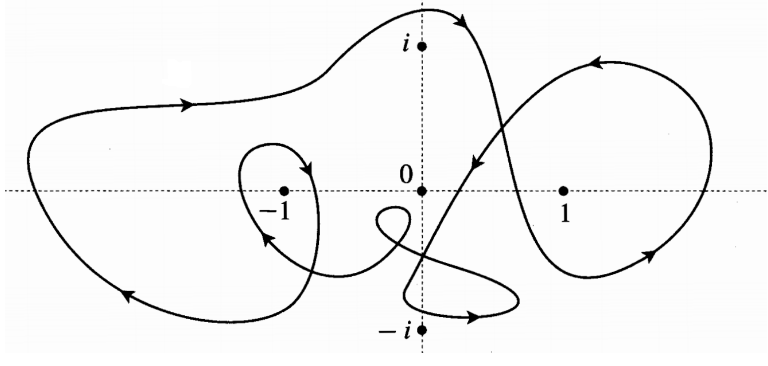
\includegraphics[width=0.6\textwidth]{image.png}
    \end{center}
\end{theorem}

\begin{proof}
    Primero factorizamos el denominador de \( f \):
    \[
        z^2 - iz - 1 - i = (z - (1+i))(z + 1).
    \]
    Luego \begin{align*}
        f(z) = \frac{A}{z - (1+i)} + \frac{B}{z + 1} & \implies z = A(z + 1) + B(z - (1+i)) \\
                                                     & \implies z = (A + B)z + (A - B(1+i))
    \end{align*}
    Por lo tanto \( f(z) = \frac{1}{(2+i)(z+1)} + \frac{1+i}{(2+i)(z - (1+i))} \) y obtenemos \begin{align*}
        I = \oint_{C} f(z) dz & = \frac{1}{2+i} \oint_{C} \frac{dz}{z+1} + \frac{1+i}{2+i} \oint_{C} \frac{dz}{z - (1+i)}.
    \end{align*}
    Donde \begin{align*}
        \oint_C \frac{dz}{z+1} = n(C, -1) 2\pi i \\
        \oint_C \frac{dz}{z - (1+i)} = n(C, 1+i) 2\pi i
    \end{align*}
    Como \( z = 1+i \) está fuera de la curva esa integral se anula y como \( z = -1 \) está dentro del lazo grande y dentro del lazo pequeño se tiene que \( n(C, -1) = -1 - 1 = -2 \) pues se recorre en sentido horario. Reemplazando los valores obtenemos el resultado de la integral I.
\end{proof}

\vspace{0.25in}

\begin{theorem}{6}
    Calcular todos los posibles valores de la integral \begin{align*}
        \oint_C \frac{dz}{z(z^2 -1)}
    \end{align*}
    para las diferentes posibilidades de curvas cerradas C suaves a trozos que no pasan por los puntos 0, 1 y -1.
\end{theorem}

\begin{proof}
    Consideremos la siguiente descomposición en fracciones simples \begin{align*}
        \frac{1}{z(z^2 - 1)} & = \frac{A}{z} + \frac{B}{z-1} + \frac{C}{z+1}       \\
                             & \implies 1 = A(z^2 - 1) + B z (z + 1) + C z (z - 1)
    \end{align*}
    Por lo tanto, \( A = -1 \), \( B = \frac{1}{2} \) y \( C = \frac{1}{2} \) y tenemos que \begin{align*}
        \oint_C \frac{dz}{z(z^2 - 1)} & = \oint_C \left( -\frac{1}{z} + \frac{1/2}{z-1} + \frac{1/2}{z+1} \right) dz                      \\
                                      & = -\oint_C \frac{dz}{z} + \frac{1}{2} \oint_C \frac{dz}{z-1} + \frac{1}{2} \oint_C \frac{dz}{z+1}
    \end{align*}
    Donde \begin{align*}
        \oint_C \frac{dz}{z} & = n(C, 0) 2\pi i, \qquad \oint_C \frac{dz}{z-1} = n(C, 1) 2\pi i \qquad \text{y} \qquad  \oint_C \frac{dz}{z+1} = n(C, -1) 2\pi i
    \end{align*}
    Luego, \begin{align*}
        \oint_C \frac{dz}{z(z^2 - 1)} & = -n(C, 0) 2\pi i + \frac{1}{2} n(C, 1) 2\pi i + \frac{1}{2} n(C, -1) 2\pi i \\
                                      & = 2\pi i \left( -n(C, 0) + \frac{n(C, 1)}{2} + \frac{n(C, -1)}{2} \right)
    \end{align*}
    Por lo tanto, los posibles valores de la integral dependen de los valores que tomen \( n(C, 0) \), \( n(C, 1) \) y \( n(C, -1) \).
\end{proof}

\clearpage

\begin{theorem}{7}
    Muestren que si \( C \) es una curva s.a.t que va del \( 0 \) al \( 1 \) sin pasar por los puntos \( i, - i\) entonces\begin{align*}
        \int_C \frac{dz}{z^2 + 1} = \frac{\pi}{4} + k \pi \qquad \text{ para algún } k \in \Z.
    \end{align*}
\end{theorem}

\begin{proof}
    Consideremos \( \Gamma \) la curva cerrada que se obtiene al unir \( C \) con la curva \( I \) que es el segmento de línea que va de \( 0 \) a \( 1 \) sobre el eje real.
    Entonces, por el teorema de la integral de curvas cerradas \begin{align*}
        \oint_{\Gamma} \frac{dz}{z^2 + 1} = \frac{1}{2i} \left(\oint_{\Gamma} \frac{dz}{z-i} + \oint_{\Gamma} \frac{dz}{z+i} \right) & = \int_C \frac{dz}{z^2 + 1} + \int_I \frac{dz}{z^2 + 1}       \\
        \frac{2\pi i}{2i} \left( n(\Gamma, i) + n(\Gamma, -i) \right)                                                                & = \int_C \frac{dz}{z^2 + 1} + \int_0^1 \frac{dx}{x^2 + 1}     \\
        \pi k                                                                                                                        & = \int_C \frac{dz}{z^2 + 1} + {\left[ \arctan(x) \right]}_0^1 \\
        \pi k - \frac{\pi}{4}                                                                                                        & = \int_C \frac{dz}{z^2 + 1}
    \end{align*}
\end{proof}

\vspace{0.25in}

\begin{theorem}{8}
    Calcular la integral \begin{align*}
        \oint_{S^1} \frac{dz}{\sin(z)}
    \end{align*}
\end{theorem}

\begin{proof}
    Sabemos que \( \sin(z) = \sum_{n \geq 0} {(-1)}^n \frac{z^{2n+1}}{(2n+1)!} \) por lo tanto \begin{align*}
        \oint_{S^1} \frac{dz}{\sin(z)} & = \oint_{S^1} \frac{dz}{\sum_{n \geq 0} {(-1)}^n \frac{z^{2n+1}}{(2n+1)!}}                                \\
                                       & = \sum_{n \geq 0} {(-1)}^n (2n+1)! \oint_{S^1} \frac{dz}{z^{2n+1}}                                        \\
                                       & = 2\pi i \quad \text{ único término no nulo es para } n = 0 \text{ y aplicamos el ejercicio 4 con } a = 0 \\
    \end{align*}
\end{proof}

\vspace{0.25in}

\begin{theorem}{9}
    Analicen si las siguientes funciones admiten un desarrollo de Laurent alrededor del punto indicado. En caso
    afirmativo, encontrarlo e indicar cuál es el anillo de convergencia del desarrollo encontrado.
    \begin{enumerate}
        \item \( \frac{e^{3z}}{(z-2^2)} \) en \( z_0 = 2 \).
        \item \( \frac{z - \sin(z)}{z^3} \) en \( z_0 = 0 \).
        \item \( \cos(1/z) \) en \( z_0 = 0 \).
        \item \( \frac{z}{(z+1)(z+2)} \) en \( z_0 = -2 \).
        \item \( \sqrt{z^2 + 1} \) en \( z_0 = 0 \).
        \item \( \frac{1}{z^2 {(z-3)}^2} \) en \( z_0 = 3 \).
    \end{enumerate}
\end{theorem}

\begin{proof}
    Recordemos que \begin{align*}
        e^{z}    & = \sum_{n \geq 0} \frac{z^n}{n!},                                \\
        \sin(z)  & = \sum_{n \geq 0} {(-1)}^n \frac{z^{2n+1}}{(2n+1)!},             \\
        \cos(z)  & = \sum_{n \geq 0} {(-1)}^n \frac{z^{2n}}{(2n)!},                 \\
        \sqrt{w} & = e^{\frac{1}{2} \log(w)} = e^{\frac{1}{2} (\ln|w| + i \arg(w))}
    \end{align*}
    \begin{enumerate}
        \item Tenemos que \( e^{3(z-2) + 6} = e^6 \sum_{n \geq 0} \frac{3^n {(z-2)}^n}{n!} \) por lo tanto
              \[
                  f(z) = e^6 \sum_{n \geq -2} \frac{3^{n+2}}{(n+2)!} {(z-2)}^n \quad \text{ con anillo de convergencia } 0 < |z-2| < \infty.
              \]
        \item \( z - sen(z) = - \sum_{n \geq 1} {(-1)}^n \frac{z^{2n+1}}{(2n+1)!} \) por lo tanto
              \[
                  f(z) = - \sum_{n \geq 1} {(-1)}^n \frac{z^{2n+1}}{(2n+1)!} \cdot \frac{1}{z^3} = - \sum_{n \geq 1} {(-1)}^n \frac{1}{(2n+1)!} z^{2n-2}
              \]
              con anillo de convergencia \( 0 < |z| < \infty \).
        \item \( \cos(1/z) = \sum_{n \geq 0} {(-1)}^n \frac{1}{(2n)!} z^{-2n} \) con anillo de convergencia \( 0 < |z| < \infty \).
        \item \( \frac{z}{(z+1)(z+2)} = -\frac{1}{z+1} + \frac{2}{z+2} \) \begin{align*}
                  f(z) & = - \frac{1}{z+2-1} + 2 \frac{1}{z+2} = -\frac{1}{1 - (z+2)} + \frac{2}{z+2} \\
                       & = - \sum_{n \geq 0} {(z+2)}^n + 2 \frac{1}{z+2}                              \\
              \end{align*}
              Sea \( a_n = \begin{cases}
                  -2, & n = -1   \\
                  -1, & n \geq 0
              \end{cases}
              \)
              Entonces \begin{align*}
                  f(z) = \sum_{n \geq -1} a_n {(z+2)}^n
              \end{align*}
        \item Si fijamos la rama principal del logaritmo, queremos que \( w = 1 + z \) no pertenezca al eje real negativo, en un torno del origen \( w \approx 1 \)
              por lo que \( \sqrt{1+z} \) es analítica en \( z = 0 \) si \( |z| < 1 \) y
              \begin{align*}
                  {(z+1)}^{1/2} & = \sum_{n \geq 0} \binom{1/2}{n} z^n    \\
                  \implies f(z) & = \sum_{n \geq 0} \binom{1/2}{n} z^{2n} \\
              \end{align*}
        \item Usando que \( w = z-3 \) obtenemos \begin{align*}
                  \frac{1}{z^2} \frac{1}{{(z-3)}^2} & = \frac{1}{{(w+3)}^2} \frac{1}{w^2} = \frac{1}{9} \frac{1}{w^2} \cdot \frac{1}{{\left( 1 + \frac{w}{3} \right)}^2} \\
                                                    & = \frac{1}{9} \frac{1}{w^2} \sum_{n \geq 0} {(-1)}^n (n+1) {\left( \frac{w}{3} \right)}^n                          \\
                                                    & = \frac{1}{9} \sum_{n \geq -2} {(-1)}^{n+2} (n+3) \frac{w^n}{3^{n+2}}                                              \\
              \end{align*}
    \end{enumerate}
\end{proof}

\vspace{0.25in}

\begin{theorem}{10}
    Desarrollen \( f(z) = \frac{1}{(z+1)(z+3)} \) en serie de Laurent válida para \begin{enumerate}
        \item \( |z| < 1 \).
        \item \( 1 < |z| < 3 \).
        \item \( |z| > 3 \).
        \item \( 0 < |z + 1| < 2 \).
    \end{enumerate}
\end{theorem}

\begin{proof}

\end{proof}

\vspace{0.25in}

Decimos que dada una función \( f: U \to \C \) tal que \( f\left(\dfrac{1}{z}\right) \) es holomorfa en un disco pinchado centrado en \( z_0 = 0 \). Si \( f(1/z) = \sum_{n \in \Z} a_n z^n \)
es el desarrollo de Laurent en el disco pinchado, decimos que \( \sum_{n \in \Z} a_n/z^n \) es el desarrollo de Laurent de \( f(z) \) alrededor de \( z_1 = \infty \).

\begin{theorem}{11}
    Desarrollen cada función en series de Laurent según lo indicado.\begin{enumerate}
        \item \( \frac{1}{z-2} \) un desarrollo alrededor de \( z_0 = 0 \) y otro alrededor de \( z_1 = \infty \).
        \item \( z^2 e^{1/z} \) un desarrollo alrededor de \( z_0 = 0 \) y otro alrededor de \( z_1 = \infty \).
    \end{enumerate}
\end{theorem}

\begin{proof}
    Notemos que \( \frac{1}{z-2} = \frac{-1}{2} \frac{1}{1 - z/2} = - \frac{1}{2} \sum_{n \geq 0} {\left( \frac{z}{2} \right)}^n \) con anillo de convergencia \( |z| < 2 \).
    Luego, para el desarrollo alrededor de \( z_1 = \infty \) consideremos \( w = 1/z \) y tenemos que \( \frac{1}{(1/w) - 2} = \frac{w}{1 - 2w} = w \sum_{n \geq 0} {(2w)}^n = \sum_{n \geq 0} 2^n w^{n+1} = \sum_{n \geq 0} 2^n \frac{1}{z^{n+1}} \)
    con anillo de convergencia \( |w| < 1/2 \) o equivalentemente \( |z| > 2 \).

    Para la otra parte, \( z^2 e^{1/z} = z^2 \sum_{n \geq 0} \frac{1}{n!} \frac{1}{z^n} = \sum_{n \geq 0} \frac{1}{n!} z^{2-n} = \sum_{m \leq 2} \frac{1}{(2-m)!} z^m \) con anillo de convergencia \( 0 < |z| < \infty \).
    Por la definición dada la serie desarrollada alrededor de \( z_1 = \infty \) es \( \sum_{n \geq 0} \frac{1}{n!} \frac{1}{z^{n-2}} = \sum_{m \leq -2} \frac{1}{(-m+2)!} \frac{1}{z^m} \) con anillo de convergencia \( 0 < |z| < \infty \).
\end{proof}

\vspace{0.25in}

\begin{theorem}{12}
    Sea \( f \) holomorfa en \( \C \setminus \{ i, 2i \} \) tal que \begin{align*}
        \text{lim}_{z \to i} |f(z)| = \text{lim}_{z \to 2i} |f(z)| = \infty
    \end{align*}
    Demuestren que el desarrollo de Laurent de \( f \) en la corona \( 1 < |z| < 2 \) tiene infinitos términos de potencias positivias y negativas de \( z \).
\end{theorem}

\begin{proof}
    Por la \textbf{Definición 5.1.3} del \emph{Conway} se tiene que tanto \( i \) como \( 2i \) son polos de \( f \), luego por la \textbf{Ecuación 5.1.9} del \emph{Conway} \[
        f(z) = \sum_{n = 1}^{N_0} \frac{a_n}{{(z-i)}^n} + \sum_{n = 0}^{N_1} \frac{b_n}{{(z - 2i)}^n} + h(z)
    \]
    donde \( h \) es una función entera que no se anula en \( i \) ni en \( 2i \). Luego, \begin{align*}
        \frac{1}{{(z-i)}^n} & = \frac{1}{z^n} \cdot \frac{1}{{\left(1 - \frac{i}{z} \right)}^n} \qquad \text{ pues |z| > 1}                                                      \\
                            & = \frac{1}{z^n} \sum_{k \geq 0} \binom{n + k - 1}{k} {\left( -\frac{i}{z} \right)}^k = \sum_{k \geq 0} \binom{n+k-1}{k} {(-i)}^k \frac{1}{z^{n+k}}
    \end{align*}
    y, por otro lado \begin{align*}
        \frac{1}{{(z-2i)}^n} & = \frac{1}{{(2i)}^n} \cdot \frac{1}{{\left( 1 - \frac{z}{2i} \right)}^n} \qquad \text{ pues |z| < 2}                                                          \\
                             & = \frac{1}{{(2i)}^n} \sum_{k \geq 0} \binom{n+k-1}{k} {\left( -\frac{z}{2i} \right)}^k = \sum_{k \geq 0} \binom{n+k-1}{k} {(-1)}^k \frac{1}{{(2i)}^{n+k}} z^k
    \end{align*}
    y por lo tanto el desarrollo de Laurent de \( f \) en la corona \( 1 < |z| < 2 \) tiene infinitos términos de potencias positivas y negativas de \( z \).
\end{proof}

\vspace{0.25in}

\begin{theorem}{13}
    Supongan que \( f \) es holomorfa en \( \C \setminus \{ 0 \} \) y satisface \begin{align*}
        |f(z)| \leq |z|^2 + \frac{1}{|z|^2} \quad \forall z \in \C \setminus \{ 0 \}
    \end{align*}
    Si \( f \) es una función impar, determinar que forma tiene \( f(z) \).
\end{theorem}

\begin{proof}
    Como \( f \) es holomorfa en \( \C \setminus \{ 0 \} \) existe el desarrollo de Laurent \begin{align*}
        f(z) = \sum_{n \in \Z} a_n z^n \qquad \text{ para } 0 < |z| < \infty
    \end{align*}
    Luego, sabemos que \begin{align*}
        a_n = \frac{1}{2 \pi i} \oint_{|z| = r} \frac{f(z)}{z^{n+1}} dz \qquad \text{ para cualquier } r > 0
    \end{align*}
    Esto nos dice que \begin{align*}
        |a_n| & = \frac{1}{2 \pi |i|} \left| \oint_{|z|=r} \frac{f(z)}{z^{n+1}} dz \right| \\
              & =\frac{2 \pi r}{2 \pi} M(r) \frac{1}{r^{n+1}}                              \\
              & = M(r) \frac{1}{r^n}
    \end{align*}
    Por la desigualdad de la hipotesis \begin{align*}
        M(r) & = \max_{|z|=r} |f(z)| \leq r^2 + \frac{1}{r^2}
    \end{align*}
    Por lo tanto, \begin{align*}
        |a_n| & \leq \frac{1}{r^{n-2}} \left( 1 + \frac{1}{r^4} \right)
    \end{align*}
    Tomando \( r \to \infty \) y \( r \to 0^{+} \) se tiene que \( a_n = 0 \) para \( n > 2 \) y \( n < -2 \). Esto nos dice que \begin{align*}
        f(z) & = a_{-2} z^{-2} + a_{-1} z^{-1} + a_0 + a_1 z + a_2 z^2
    \end{align*}
    y usando que \( f \) es impar podemos concluir que \( a_{-2} = a_0 = a_2 = 0 \). Por lo tanto, \begin{align*}
        f(z) & = a_{-1} z^{-1} + a_1 z
    \end{align*}
\end{proof}

\vspace{0.25in}

\begin{theorem}{14}
    Encuentren todas las funciones holomorfas en \( \C \setminus \{ 0 \} \) tales que \begin{align*}
        \lim_{z \to 0} z f(z) = 1 \qquad \text{y} \qquad \lim_{|z| \to \infty} f(z) = 1
    \end{align*}
\end{theorem}

\begin{proof}
    Análogamente al ejercicio anterior \( f \) admite un desarrollo en serie de Laurent de la forma \begin{align*}
        f(z) = \sum_{n \in \Z} a_n z^n \qquad \text{ para } 0 < |z| < \infty
    \end{align*}
    y usando la hipotesis de que \( \lim_{z \to 0} z f(z) = 1 \) se tiene que \begin{align*}
        \sum_{n \in \Z} a_n z^{n+1} & \to 1 \qquad \text{ cuando } z \to 0                                             \\
        \implies a_{-1}             & = 1 \qquad \text{y } a_n = 0 \text{ para } n < -1 \text{ pues si no divergería.}
    \end{align*}
    Por otro lado, \begin{align*}
        a_n   & = \frac{1}{2 \pi i } \oint_{|z| = r} \frac{f(z)}{z^{n+1}} dz \qquad \text{ para cualquier } r > 0                                              \\
        |a_n| & = \frac{1}{2 \pi |i|} \left| \oint_{|z|=r} \frac{f(z)}{z^{n+1}} dz \right| = \frac{2 \pi r}{2 \pi} M(r) \frac{1}{r^{n+1}} = M(r) \frac{1}{r^n}
    \end{align*}
    haciendo tender \( r \to \infty \) si \( n > 0 \) se tiene que \( a_n = 0 \) pues \( M(r) \to 1 \) y nos queda ver que ocurre con \( a_0 \), como \( f(z) \to 1 \) cuando \( |z| \to +\infty \) el termino \( a_0 \) debe ser igual a \( 1 \).
    Por lo tanto, la única función que cumple las condiciones es \begin{align*}
        f(z) & = \frac{1}{z} + 1
    \end{align*}
    que es holomorfa en \( \C \setminus \{ 0 \} \).
\end{proof}
\end{document}